% section | subsection | subsubsection | paragraph | subparagraph | verbatim | enumerate | item

% Just let it be an Article bro
\documentclass{article}

% Cover Metadata
\title{Programming in Python}
\date{31 Oct 2025}
\author{Maulana Hafidz Ismail}

% Equation Setup
\usepackage{amsmath}

% Image Setup
\usepackage{graphicx}
\usepackage{float}

% Link Setup
\usepackage{hyperref}

% Highlighting Setup
\usepackage{soul}
\usepackage{xcolor}
\sethlcolor{red!30}
\newcommand{\hlblue}[1]{\sethlcolor{cyan!30}\hl{#1}\sethlcolor{yellow}}

% Line Width
\sloppy
\setlength{\emergencystretch}{3em}
\hbadness=99999

\usepackage{tabularx}

% Code Syntax Setup
\usepackage{listings}
\usepackage{xcolor} % untuk warna
\lstset{
basicstyle=\ttfamily\small,
frame=single,
breaklines=true,
backgroundcolor=\color{gray!10},
keywordstyle=\color{blue},
commentstyle=\color{gray},
stringstyle=\color{red},
tabsize=2,
captionpos=b
}

% Start of the Article
\begin{document}

% Cover Page
\pagenumbering{gobble}
\maketitle
\newpage

% Table of Content Page
\tableofcontents
\newpage
\pagenumbering{arabic}

% Main Content
\section{Memulai dengan Python}
\subsection{Tentang Python}
Python dinamai setelah acara TV "Monty Python's Flying Circus" dan bukan dari ular piton. Nama ini dipilih karena dianggap singkat dan misterius. Python digunakan dalam aplikasi yang sering kita gunakan, seperti Instagram, Facebook, Google, dan Spotify. Contoh penggunaan Python dalam machine learning termasuk TensorFlow, yang digunakan oleh Airbnb untuk mengklasifikasikan gambar dan oleh perusahaan kesehatan untuk mengklasifikasikan data MRI. Python dianggap mudah digunakan dan sederhana, dengan banyak pustaka (libraries) yang mendukung pengembangan. Memungkinkan pengembang untuk membuat fitur dengan cepat dan melihat hasilnya lebih cepat.

\subsection{Sejarah Pemrograman}
\begin{itemize}
    \item Charles Babbage, pada tahun 1822, menciptakan difference engine untuk mengurangi kesalahan manusia dalam perhitungan.
    \item Babbage juga mengembangkan analytical engine, yang dianggap sebagai dasar dari komputer modern.
    \item Teman Babbage, Ada Lovelace, menulis dokumen yang menjelaskan bagaimana analytical engine dapat melakukan urutan perhitungan, mirip dengan apa yang dilakukan oleh program komputer.
\end{itemize}

\subsection{Dasar-dasar Pemrograman}
\begin{itemize}
    \item Komputer hanya memahami binary code, yang terdiri dari dua digit: 0 dan 1. Binary Code: Sistem bilangan yang hanya menggunakan dua angka, 0 (off) dan 1 (on).
    \item Setiap program yang ditulis harus dikonversi menjadi machine code (kode mesin) agar dapat dipahami oleh komputer. Contoh konversi: Decimal 1 menjadi Binary 1, Decimal 2 menjadi Binary 10.
    \item Komputer menggunakan transistors untuk merepresentasikan binary code. Transistor: Komponen elektronik yang berfungsi sebagai saklar untuk mengontrol aliran listrik.
\end{itemize}

\subsection{Apa itu Pemrograman?}
Pemrograman adalah kemampuan untuk memberikan serangkaian instruksi kepada komputer dalam bahasa yang dapat dipahami.

Pemrograman adalah keterampilan yang dapat diasah dengan latihan. Semakin sering berlatih, semakin baik kemampuan pemrograman seseorang.

Pemrograman juga merupakan keterampilan kreatif, karena ada banyak cara untuk menyelesaikan masalah dengan menulis program.

\subsection{Manfaat Belajar Python}
\begin{itemize}
    \item Mudah Dipelajari: Python memiliki sintaks yang mirip dengan bahasa Inggris, sehingga lebih mudah dibaca dan dipahami.
    \item Produktivitas Tinggi: Dengan Python, pengembang dapat menyelesaikan proyek lebih cepat karena sintaks yang sederhana dan memerlukan lebih sedikit kode dibandingkan dengan bahasa lain seperti C atau Java.
\end{itemize}

\subsection{Aplikasi Python}
\begin{itemize}
    \item Berbagai Platform: Python dapat digunakan di Windows, Mac, dan Linux.
    \item Bidang Penggunaan: Python banyak digunakan dalam pengembangan web, kecerdasan buatan, machine learning, analisis data, dan aplikasi pemrograman lainnya.
\end{itemize}

\subsection{Menjalankan Python di Command Line}
\begin{itemize}
    \item Python Shell:

          Ini adalah cara pertama untuk menjalankan program Python. Shell ini berguna untuk menjalankan dan menguji skrip kecil tanpa perlu membuat file baru dengan ekstensi .PY. Anda dapat mengetikkan potongan kode langsung di shell.

          Cukup ketik python di command line untuk membuka Python shell, lalu masukkan kode yang ingin dijalankan.

    \item Menjalankan File Python

          Cara kedua adalah menjalankan file Python langsung dari command line. Setiap file dengan ekstensi .PY dapat dijalankan dengan perintah tertentu.

          Ketik python \verb|nama_file.py| di command line untuk menjalankan file tersebut.
\end{itemize}

\subsection{Sintaksis Python dan Pentingnya Spasi}
Menggunakan print("Hello") untuk menghasilkan teks. \verb|print| adalah fungsi yang digunakan untuk menampilkan output ke layar.

\begin{lstlisting}[language=Python, caption={}, captionpos=b]
print("Hello") print("World")
\end{lstlisting}

Jika mencoba menulis dua pernyataan print dalam satu baris tanpa pemisah, akan muncul error \verb|SyntaxError: invalid syntax|. SyntaxError adalah kesalahan yang terjadi ketika kode tidak mengikuti aturan sintaks yang benar.

Mengatasi Error:
\begin{itemize}
    \item Metode Pertama: Memindahkan pernyataan print kedua ke baris baru.
          \begin{lstlisting}[language=Python, caption={}, captionpos=b]
print("Hello")
print("World")
    \end{lstlisting}
    \item Metode Kedua: Memisahkan pernyataan dengan titik koma.

          \begin{lstlisting}[language=Python, caption={}, captionpos=b]
print("Hello"); print("World")
    \end{lstlisting}
\end{itemize}

\paragraph{Whitespace adalah} karakter kosong (spasi, tab, newline) yang tidak terlihat tetapi mempengaruhi struktur kode. Menambahkan spasi di sekitar operator tidak menyebabkan masalah, tetapi menambahkan baris baru bisa menyebabkan error. Contohnya seperti ini:
\begin{lstlisting}[language=Python, caption={}, captionpos=b]
#any ammount of whitespace on a single line is ok
x     =        1        +        2
\end{lstlisting}
Dan berikut tidak benar:
\begin{lstlisting}[language=Python, caption={}, captionpos=b]
x = 1
+ 2

\end{lstlisting}

\paragraph{Indentasi adalah} penggunaan spasi atau tab untuk mengatur blok kode, yang menunjukkan hierarki dan struktur. Penting untuk struktur kontrol seperti if statement.
\begin{lstlisting}[language=Python, caption={}, captionpos=b]
if name == "John":
    print(name)
\end{lstlisting}
Jika indentasi dihapus, akan muncul error \verb|IndentationError: expected an indented block|.

\subsection{Memberi Komentar pada Kode}
Menambahkan komentar ke kode tidak hanya membantu Anda sebagai pengembang, tetapi juga membantu anggota tim lainnya. Komentar sangat berguna untuk menyegarkan ingatan Anda tentang kode yang mungkin telah Anda tulis berbulan-bulan lalu dan Anda mungkin lupa apa tujuannya. Ada beberapa alasan mengapa Anda perlu menambahkan komentar ke berkas kode. Alasannya antara lain:
\begin{itemize}
    \item Menjelaskan tujuan kode.
    \item Memberitahu pengembang bahwa kode tersebut sudah usang.
    \item Menambahkan komentar TODO untuk pekerjaan yang akan diselesaikan nanti.
\end{itemize}
Berikut adalah contoh berbagai jenis komentar yang dapat digunakan.

\subsubsection{Single-line comments}
Penggunaan simbol \verb|#| memberi tahu Python untuk mengabaikan semua yang ada setelah titik ini hingga akhir baris saat ini.
\begin{lstlisting}[language=Python, caption={}, captionpos=b]
# Don't try to Run Me, I'm a comment
x = 10
\end{lstlisting}

\subsubsection{Multi-line comments}
\paragraph{Tanda Kutip Tiga (''' atau """):} Python menggunakan tanda kutip tunggal atau ganda tiga kali untuk membuat komentar multi-baris. Tanda kutip ini biasanya digunakan untuk docstring atau komentar yang mencakup beberapa baris.

\subsubsection{Inline comments}
Simbol \verb|#| memberi tahu Python untuk mengabaikan semua yang ada setelah titik ini hingga akhir baris saat ini. Hal ini memungkinkan komentar ditempatkan di dalam kode itu sendiri. Komentar sebaris sebaiknya digunakan untuk memberikan informasi penting tentang kode yang ditanganinya.

\begin{lstlisting}[language=Python, caption={}, captionpos=b]
x = 1  # Resetting buffer size
\end{lstlisting}

Ingatlah untuk selalu memiliki alasan untuk berkomentar, komentar harus memberikan informasi kepada pembaca dan tidak mengganggu.

\subsection{Pengertian Variabel}
Variabel adalah tempat untuk menyimpan data yang dapat berubah. Dalam Python, Anda dapat mendeklarasikan variabel dengan memberikan nama dan nilai.

Contoh sintaks: X = 10 (di mana X adalah nama variabel dan 10 adalah nilainya).

\subsection{Penamaan Variabel}
Penting untuk memberikan nama yang bermakna agar mudah dipahami oleh programmer lain.

Dua konvensi penamaan yang umum digunakan:
\begin{itemize}
    \item \verb|camelCase|: Huruf pertama dari kata pertama kecil, dan huruf pertama dari setiap kata berikutnya besar. Contoh: \verb|myName|.
    \item \verb|snake_case|`': Semua huruf kecil dengan garis bawah sebagai pemisah. Contoh: \verb|my_name|.
\end{itemize}

\subsection{Mengubah dan Menghapus Variabel}
Anda dapat mengubah nilai variabel yang sudah dideklarasikan dengan cara mendeklarasikannya kembali.
\begin{lstlisting}[language=Python, caption={}, captionpos=b]
a = 10
print(a)  # Output: 10
a = 5
print(a)  # Output: 5
\end{lstlisting}

Untuk menghapus variabel, gunakan perintah del.
\begin{lstlisting}[language=Python, caption={}, captionpos=b]
del a
print(a)  # Akan menghasilkan error: NameError: name 'a' is not defined
\end{lstlisting}

\subsection{Deklarasi Beberapa Variabel}
Anda dapat mendeklarasikan beberapa variabel sekaligus.
\begin{lstlisting}[language=Python, caption={}, captionpos=b]
a, b, c = 1, 2, 3
print(a, b, c)  # Output: 1 2 3
\end{lstlisting}

\subsection{Tipe Data dalam Python}
Tipe data adalah atribut yang terkait dengan data yang memberi tahu sistem komputer bagaimana menginterpretasikan nilainya.

Tipe Data memastikan data dikumpulkan dalam format yang diinginkan dan nilai setiap properti sesuai harapan.

\subsection{Jenis Tipe Data Utama}
\begin{figure}[H]
    \centering
    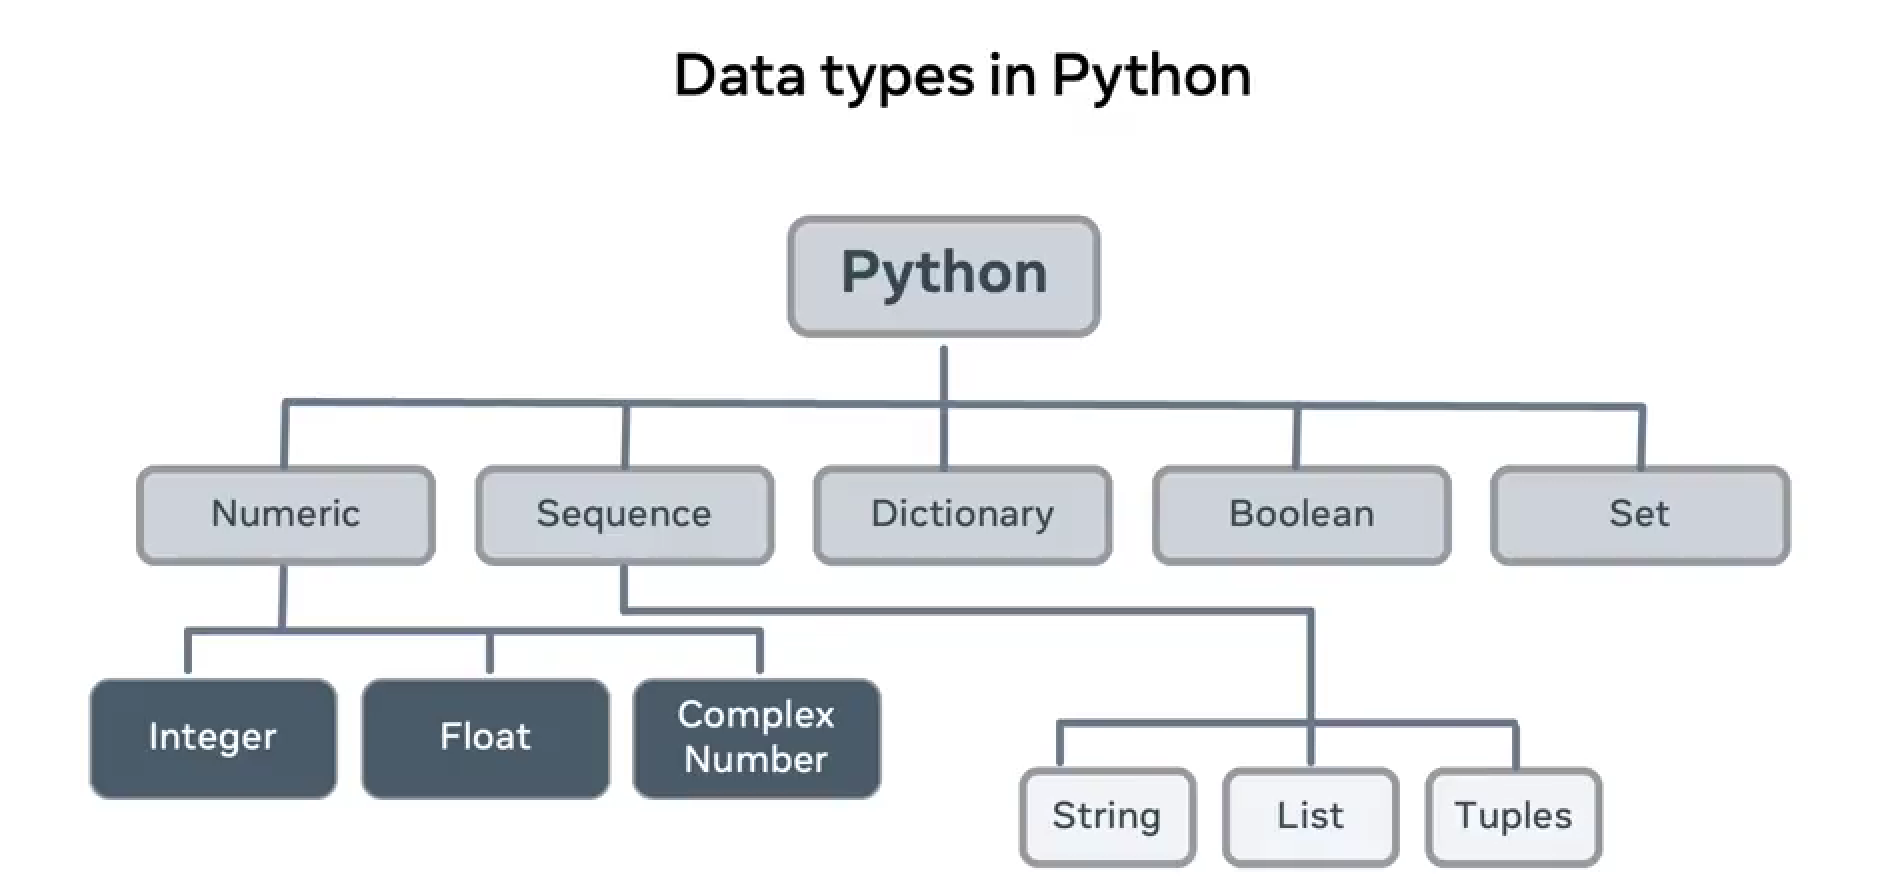
\includegraphics[width=0.8\textwidth]{./Picts/data-types.png}
    \caption{Pohon Tipe Data}
\end{figure}
\begin{itemize}
    \item Numeric: Tipe data ini mencakup:
          \begin{itemize}
              \item Integer: Angka bulat tanpa desimal, misalnya 10 atau -10.
              \item Float: Angka dengan desimal, misalnya 10.5 atau 6.7.
              \item Complex: Angka kompleks yang terdiri dari bagian nyata dan imajiner, misalnya a = 10 + 10j.
          \end{itemize}
    \item Sequence: Tipe data yang berisi satu atau lebih tipe dalam urutan yang teratur, termasuk:
          \begin{itemize}
              \item String: Sekuens karakter yang diapit oleh tanda kutip, misalnya "Hello".
              \item List: Sekuens yang dapat berisi berbagai tipe, diapit oleh tanda kurung siku, misalnya [1, 2, 3].
              \item Tuple: Mirip dengan list, tetapi tidak dapat diubah (immutable), diapit oleh tanda kurung, misalnya (1, 2, 3).
          \end{itemize}
    \item Dictionary: Menyimpan data dalam struktur objek key-value. Contoh:
          \begin{lstlisting}[language=Python, caption={}, captionpos=b]
ed = {'a': 22, 'b': 44.4}
\end{lstlisting}
    \item Boolean: Tipe data yang hanya memiliki dua nilai, yaitu True atau False. Contoh:
          \begin{lstlisting}[language=Python, caption={}, captionpos=b]
is_valid = True
\end{lstlisting}
    \item Set: Koleksi tidak terurut dari nilai yang tidak diulang. Contoh:
          \begin{lstlisting}[language=Python, caption={}, captionpos=b]
example_set = {1, 2, 3, 4}
\end{lstlisting}
\end{itemize}

\subsection{Menentukan Tipe Data}
Fungsi \verb|type()|: Digunakan untuk menentukan tipe data dari variabel. Contoh:
\begin{lstlisting}[language=Python, caption={}, captionpos=b]
a = 10
print(type(a))  # Output: <class 'int'>
\end{lstlisting}

\subsection{Deklarasi Strings}
String adalah sekuens karakter yang dikelilingi oleh tanda kutip tunggal (' ') atau ganda (" "). Contoh sintaks: \verb|a = 'hello' atau b = "hello"|.

Encoding adalah proses mengubah karakter menjadi bentuk yang dapat dipahami komputer. Python menggunakan \verb|Unicode| untuk encoding.

\subsection{Mengakses dan Mengubah String}
\begin{itemize}
    \item Indexing: Setiap karakter dalam string dapat diakses menggunakan indeks. Python menggunakan zero-indexing, artinya indeks dimulai dari 0. Contoh: \verb|name[0]| mengakses karakter pertama.
    \item Mengubah Nilai: Anda dapat mengubah nilai string dengan cara menetapkan nilai baru ke variabel. Contoh: name = 'Paul'.
\end{itemize}

\subsection{Fungsi dan Operasi pada Strings}
\begin{itemize}
    \item \verb|len()|: Fungsi untuk memeriksa panjang string. Contoh sintaks: \verb|len(name)| akan mengembalikan jumlah karakter dalam string.
    \item Concatenation: Menggabungkan dua string menggunakan operator +. Contoh: \verb|a + b| akan menggabungkan string a dan b.
\end{itemize}

\subsection{Contoh Penggunaan}
\begin{itemize}
    \item Single Line String: \verb|a = 'this is a single line'|
    \item Multi-Line String: Untuk membuat string yang panjang, gunakan backslash (\verb|\|) di akhir baris. Contoh:
          \begin{lstlisting}[language=Python, caption={}, captionpos=b]
b = 'this is a multi-line string example \
that continues here.'
\end{lstlisting}
    \item Output: Menggunakan print() untuk menampilkan string. Contoh: print(a) akan mencetak nilai dari a.
\end{itemize}

\subsection{Cheatsheets Tipe Data dan Fungsi}
Berikut ini adalah panduan singkat tentang jenis data dalam Python.
\subsubsection{Tipe Data}
\begin{tabularx}{\textwidth}{|X|X|X|}
    \hline
    \textbf{Tipe Data} & \textbf{Meaning} & \textbf{Example}       \\
    \hline
    string             & Text             & 'Hello', "Testing 123" \\
    \hline
    integer            & Numbers          & -5, 4, 3, 2, 0         \\
    \hline
    float              & Decimals         & 2.4, 5.2, 1000.00      \\
    \hline
\end{tabularx}

\subsubsection{Flow Control}
Operator Perbandingan

\begin{tabularx}{\textwidth}{|X|X|X|}
    \hline
    \textbf{Operator} & \textbf{Meaning}         & \textbf{Example} \\
    \hline
    ==                & Equals                   & a == b           \\
    \hline
    !=                & Not Equal                & a != b           \\
    \hline
    <                 & Less than                & a < b            \\
    \hline
    >                 & Greater than             & a > b            \\
    \hline
    <=                & Less than or Equal to    & a <= b           \\
    \hline
    >=                & Greater than or Equal to & a >= b           \\
    \hline
\end{tabularx}

\subsubsection{Indentasi}
Indentasi digunakan untuk mendefinisikan blok kode dalam Python. Berbeda dengan banyak bahasa pemrograman yang menggunakan kurung kurawal {} untuk mengelompokkan kode, Python menggunakan indentasi.

Indentasi wajib digunakan dalam Python dan digunakan untuk menunjukkan pernyataan mana yang termasuk dalam loop, fungsi, kondisional, dan struktur lainnya.
\begin{lstlisting}[language=Python, caption={}, captionpos=b]
if x > 0:  # Colon indicates the start of the block
    print("Positive")  # Indented 
else:
    print("Non-positive") # Indented
\end{lstlisting}

\subsubsection{Komentar}
Menempatkan simbol \verb|#| di depan teks yang ingin Anda jadikan komentar akan membuat Python mengabaikan semua teks dari titik tersebut hingga akhir baris saat ini.

Triple Quotes \verb|(''' or """)|: Python menggunakan tanda kutip tunggal atau ganda bertiga untuk membuat komentar \verb|multi-baris|. Tanda kutip ini umumnya digunakan untuk docstrings atau komentar yang mencakup beberapa baris.

Simbol \verb|#| akan membuat Python mengabaikan semua teks mulai dari titik tersebut hingga akhir baris saat ini, sehingga komentar inline dapat dibuat dengan cara ini.

Kolon \verb|(:)|: Digunakan untuk menandai awal blok kode, seperti dalam perulangan, kondisi, dan definisi fungsi.

\begin{lstlisting}[language=Python, caption={}, captionpos=b]
# Single Line comment

# This is a multiline comment
# which can be used for long comments

x = 1 # assigns value of 1 to x

if x > 0:  # Colon starts the block
    print("Positive")
\end{lstlisting}

\subsubsection{Built-in Functions}
\begin{itemize}
    \item \verb|print()|

          Fungsi ini mencari perangkat output default, terminal Anda, dan menampilkan nilai yang diteruskan kepadanya.
          \begin{lstlisting}[language=Python, caption={}, captionpos=b]
    print("Hello")
    \end{lstlisting}
    \item \verb|input()|

          Fungsi ini mencari perangkat input default, yaitu keyboard Anda, dan menangkap nilainya. Nilai ini kemudian dapat ditugaskan atau digunakan.
          \begin{lstlisting}[language=Python, caption={}, captionpos=b]
    print("Where do you live?")
    location = input()
    print("So you live in " + location)
    \end{lstlisting}
          Catatan: Blok kode di atas akan menampilkan prompt kepada pengguna dengan pertanyaan "Di mana Anda tinggal?". Pengguna kemudian akan memasukkan respons dan menekan tombol Return untuk melanjutkan eksekusi kode yang tersisa. Respons yang dimasukkan oleh pengguna disimpan, dikembalikan sebagai output, atau dapat ditugaskan ke variabel tertentu tergantung pada konteks penggunaannya.
    \item \verb|len()|

          Fungsi ini mengembalikan panjang atau jumlah elemen yang terdapat dalam struktur yang diterapkan padanya. Struktur tersebut dapat berupa string, array, daftar, tuple, kamus, atau urutan apa pun.
          \begin{lstlisting}[language=Python, caption={}, captionpos=b]
    len("Hello")
    5
    \end{lstlisting}
    \item \verb|str()|

          Fungsi ini dapat digunakan untuk mengubah nilai yang diberikan menjadi String.
          \begin{lstlisting}[language=Python, caption={}, captionpos=b]
    str(55)
    '55'
    \end{lstlisting}
    \item \verb|int()|

          Fungsi ini dapat digunakan untuk mengubah nilai yang diberikan menjadi bilangan bulat.
          \begin{lstlisting}[language=Python, caption={}, captionpos=b]
    int('75')
    75
    \end{lstlisting}
    \item \verb|float()|

          Fungsi ini dapat digunakan untuk mengubah nilai yang diberikan menjadi bilangan float.
          \begin{lstlisting}[language=Python, caption={}, captionpos=b]
    some_int = 10
    float(some_int)
    10.0
    \end{lstlisting}
\end{itemize}

\subsubsection{Membuat Fungsi}
Fungsi dalam Python memerlukan kata kunci untuk mendefinisikannya: `def` diikuti oleh identifikasi (nama), yang membentuk tanda tangan fungsi. Tubuh fungsi berisi kode yang akan dijalankan saat fungsi dipanggil.
\begin{lstlisting}[language=Python, caption={}, captionpos=b]
def say_hello():
    return "Hello there!"

# With parameters
def say_hello(you):
    return "Hello " +  you
\end{lstlisting}

\subsection{Apa itu Typecasting?}
Typecasting adalah proses mengubah satu tipe data menjadi tipe data lain. Dalam Python, ada dua jenis konversi: implicit dan explicit.

\subsection{Implicit Type Conversion}
\paragraph{Implicit Conversion}: Dilakukan secara otomatis oleh compiler Python untuk mencegah kehilangan data. Contoh: mengubah int menjadi float jika nilai yang dimasukkan adalah desimal.

Penting untuk dicatat bahwa Python hanya dapat mengonversi nilai jika tipe data tersebut kompatibel. Misalnya, int dan float kompatibel, tetapi String dan int tidak.

\subsection{Explicit Type Conversion}
\paragraph{Explicit Conversion}: Dilakukan oleh pengembang menggunakan fungsi yang disediakan oleh Python. Beberapa
\begin{itemize}
    \item \verb|str()|: Mengubah tipe data menjadi string. Sintaks: \verb|str(value)|.
    \item \verb|int(): Mengubah tipe data menjadi integer. Sintaks: \verb|int(value)|.
    \item \verb|float()|: Mengubah tipe data menjadi float. Sintaks: \verb|float(value)|.
\end{itemize}

\subsection{Fungsi Typecasting Lainnya}
\begin{itemize}
    \item \verb|ord()|: Mengembalikan integer yang mewakili karakter unicode yang mendasarinya.
    \item \verb|hex()|: Mengonversi integer menjadi string heksadesimal.
    \item \verb|oct()|: Mengambil integer dan mengembalikan string yang mewakili angka oktal.
    \item \verb|tuple(), set(), list(), dict()|: Fungsi lain untuk mengonversi tipe data.
\end{itemize}


\newpage

\section{Dasar Progrramming dengan Python}


\newpage

\section{Paradigma Pemrograman}


\newpage

\section{Modul, Paket, Pustaka, and Alat-alat}


\newpage


% End of Main Content
\end{document}